\documentclass{article}\usepackage[]{graphicx}\usepackage[]{color}
% maxwidth is the original width if it is less than linewidth
% otherwise use linewidth (to make sure the graphics do not exceed the margin)
\makeatletter
\def\maxwidth{ %
  \ifdim\Gin@nat@width>\linewidth
    \linewidth
  \else
    \Gin@nat@width
  \fi
}
\makeatother

\definecolor{fgcolor}{rgb}{0.345, 0.345, 0.345}
\newcommand{\hlnum}[1]{\textcolor[rgb]{0.686,0.059,0.569}{#1}}%
\newcommand{\hlstr}[1]{\textcolor[rgb]{0.192,0.494,0.8}{#1}}%
\newcommand{\hlcom}[1]{\textcolor[rgb]{0.678,0.584,0.686}{\textit{#1}}}%
\newcommand{\hlopt}[1]{\textcolor[rgb]{0,0,0}{#1}}%
\newcommand{\hlstd}[1]{\textcolor[rgb]{0.345,0.345,0.345}{#1}}%
\newcommand{\hlkwa}[1]{\textcolor[rgb]{0.161,0.373,0.58}{\textbf{#1}}}%
\newcommand{\hlkwb}[1]{\textcolor[rgb]{0.69,0.353,0.396}{#1}}%
\newcommand{\hlkwc}[1]{\textcolor[rgb]{0.333,0.667,0.333}{#1}}%
\newcommand{\hlkwd}[1]{\textcolor[rgb]{0.737,0.353,0.396}{\textbf{#1}}}%
\let\hlipl\hlkwb

\usepackage{framed}
\makeatletter
\newenvironment{kframe}{%
 \def\at@end@of@kframe{}%
 \ifinner\ifhmode%
  \def\at@end@of@kframe{\end{minipage}}%
  \begin{minipage}{\columnwidth}%
 \fi\fi%
 \def\FrameCommand##1{\hskip\@totalleftmargin \hskip-\fboxsep
 \colorbox{shadecolor}{##1}\hskip-\fboxsep
     % There is no \\@totalrightmargin, so:
     \hskip-\linewidth \hskip-\@totalleftmargin \hskip\columnwidth}%
 \MakeFramed {\advance\hsize-\width
   \@totalleftmargin\z@ \linewidth\hsize
   \@setminipage}}%
 {\par\unskip\endMakeFramed%
 \at@end@of@kframe}
\makeatother

\definecolor{shadecolor}{rgb}{.97, .97, .97}
\definecolor{messagecolor}{rgb}{0, 0, 0}
\definecolor{warningcolor}{rgb}{1, 0, 1}
\definecolor{errorcolor}{rgb}{1, 0, 0}
\newenvironment{knitrout}{}{} % an empty environment to be redefined in TeX

\usepackage{alltt}

\usepackage{float}

% Set the margins on the page to not be so large
\addtolength{\oddsidemargin}{-.875in}
\addtolength{\evensidemargin}{-.875in}
\addtolength{\textwidth}{1.75in}
\addtolength{\topmargin}{-.875in}
\addtolength{\textheight}{1.75in}

% Take off page numbering
\pagenumbering{gobble}
\IfFileExists{upquote.sty}{\usepackage{upquote}}{}
\begin{document}

\title{%
  4.1.1: R - Penalized Regression Methods \\
  (Ridge Regression, LASSO, and Elastic Net) \\
  \smallskip
  \large Stat 5100: Dr. Bean
}
\date{}

\maketitle

\textbf{Example: } (Ridge Regression; recall Handout 2.6.1 example) A study seeks to relate (in females) amount of body fat ($Y$) to triceps skinfold thickness ($X_1$), thigh circumference ($X_2$), and midarm circumference ($X_3$).  Amount of body fat is expensive to measure, requiring immersion of person in water.  This expense motivates the desire for a predictive model based on these inexpensive predictors.

\begin{knitrout}
\definecolor{shadecolor}{rgb}{0.969, 0.969, 0.969}\color{fgcolor}\begin{kframe}
\begin{alltt}
\hlcom{# Load the data}
\hlkwd{library}\hlstd{(stat5100)}
\hlkwd{data}\hlstd{(bodyfat)}

\hlcom{# Look at the original fit along with VIF:}
\hlstd{bodyfat_lm} \hlkwb{<-} \hlkwd{lm}\hlstd{(body} \hlopt{~} \hlstd{triceps} \hlopt{+} \hlstd{thigh} \hlopt{+} \hlstd{midarm,} \hlkwc{data} \hlstd{= bodyfat)}
\hlstd{olsrr}\hlopt{::}\hlkwd{ols_vif_tol}\hlstd{(bodyfat_lm)}
\end{alltt}
\begin{verbatim}
##   Variables   Tolerance      VIF
## 1   triceps 0.001410750 708.8429
## 2     thigh 0.001771971 564.3434
## 3    midarm 0.009559681 104.6060
\end{verbatim}
\begin{alltt}
\hlcom{# Try ridge regression as a remedial measure}
\hlcom{# -----------------------------------------}
\hlcom{# We use the ridge() function inside the genridge package to do this. Note that}
\hlcom{# instead of specifying our model using a formula (formulas in R are of the}
\hlcom{# form Y ~ X1 + X2 + X3), we create a dataframe of just our predictor variables}
\hlcom{# and a vector of our response variable. There are many great packages to}
\hlcom{# perform ridge regression with, but this one was selected for this course}
\hlcom{# due to the greater plotting features available in this particular package.}
\hlstd{y} \hlkwb{<-} \hlstd{bodyfat}\hlopt{$}\hlstd{body}

\hlcom{# Our X must come in the form of a matrix. First we take out the "body" column}
\hlcom{# from the dataframe, and then we convert it to a matrix.}
\hlstd{X} \hlkwb{<-} \hlkwd{as.matrix}\hlstd{(}\hlkwd{subset}\hlstd{(bodyfat,} \hlkwc{select} \hlstd{=} \hlopt{-}\hlstd{body))}

\hlcom{# Range of lambda values to try}
\hlstd{lambda_seq} \hlkwb{<-} \hlkwd{seq}\hlstd{(}\hlnum{0}\hlstd{,} \hlnum{0.04}\hlstd{,} \hlkwc{by} \hlstd{=} \hlnum{0.005}\hlstd{)}

\hlcom{# Create the model and plot to check for an optimal value of lambda}
\hlstd{bodyfat_test_ridge_lm} \hlkwb{<-} \hlstd{genridge}\hlopt{::}\hlkwd{ridge}\hlstd{(y, X,} \hlkwc{lambda} \hlstd{= lambda_seq)}
\hlstd{stat5100}\hlopt{::}\hlkwd{ridge_vif_trace_plot}\hlstd{(bodyfat_test_ridge_lm)}
\end{alltt}
\end{kframe}

{\centering 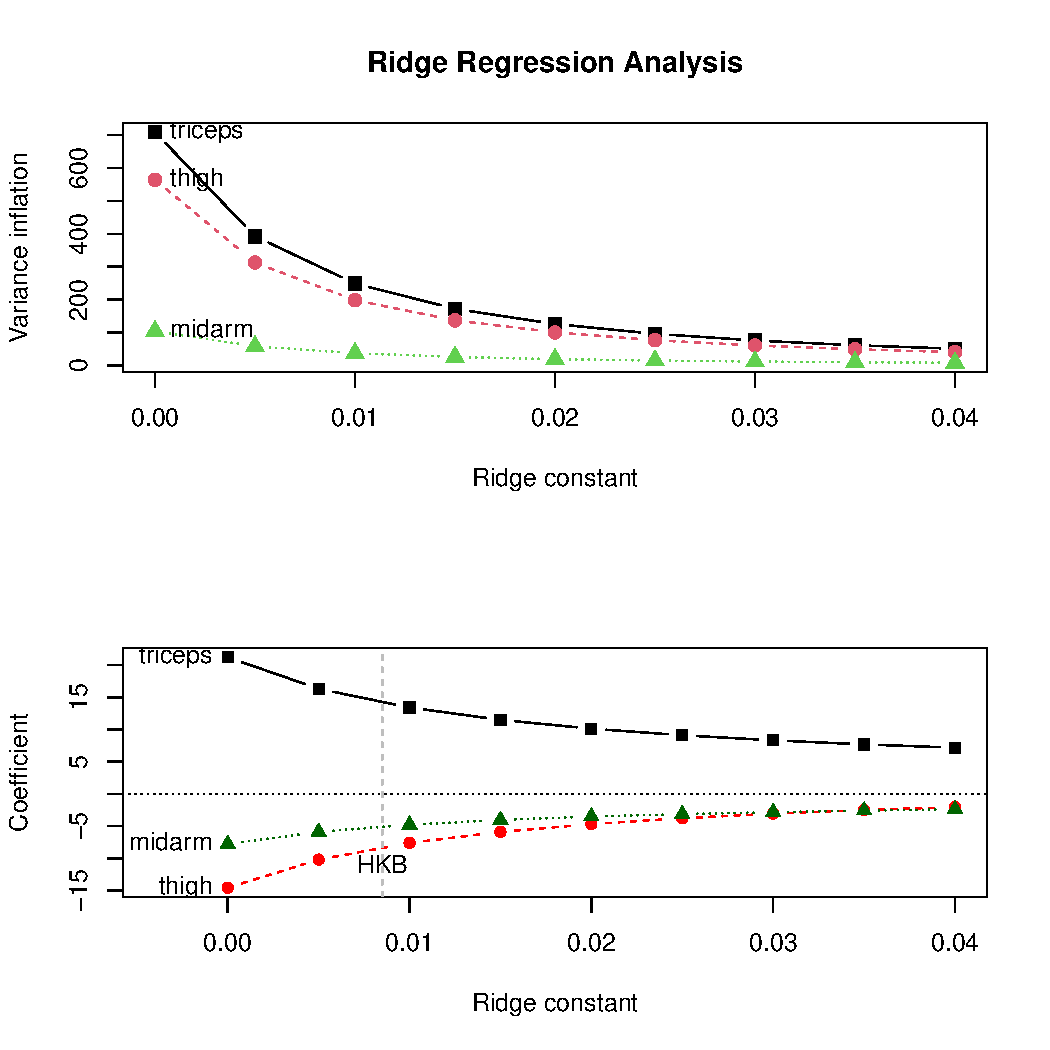
\includegraphics[width=0.6\textwidth]{figure/unnamed-chunk-1-1} 

}


\begin{kframe}\begin{alltt}
\hlstd{a} \hlkwb{<-} \hlstd{glmnet}\hlopt{::}\hlkwd{glmnet}\hlstd{(X, y,} \hlkwc{alpha} \hlstd{=} \hlnum{0}\hlstd{,} \hlkwc{lambda} \hlstd{= lambda_seq)}
\end{alltt}
\end{kframe}
\end{knitrout}

The plot on top is the VIF plot, and the plot on the bottom is the ridge trace plot. We look for the smallest ridge constant such that the VIF is ``small enough'' (roughly around 1 if possible) and the coefficient estimates have become ``stable'' (usually implying that the coefficient estimate curve has leveled off)

Here, we will pick $\lambda = 0.02$. Let's fit a model with this ridge constant and then look at the coefficient estimates.

\begin{knitrout}
\definecolor{shadecolor}{rgb}{0.969, 0.969, 0.969}\color{fgcolor}\begin{kframe}
\begin{alltt}
\hlstd{bodyfat_ridge_lm} \hlkwb{<-} \hlstd{genridge}\hlopt{::}\hlkwd{ridge}\hlstd{(y, X,} \hlkwc{lambda} \hlstd{=} \hlnum{0.02}\hlstd{)}
\hlstd{bodyfat_ridge_lm}\hlopt{$}\hlstd{coef}
\end{alltt}
\begin{verbatim}
##       triceps     thigh   midarm
## 0.02 10.12698 -4.682273 -3.52701
\end{verbatim}
\end{kframe}
\end{knitrout}

\end{document}
